\documentclass[11pt,a4paper,oneside]{book}
\usepackage[hmargin={1.25in,1.25in},vmargin={1.25in,1.25in}]{geometry}

\makeindex
\usepackage{textcomp}
\usepackage{fancyhdr}
\usepackage{makeidx}
\pagestyle{myheadings}
\fancyhf{}
\rhead[\leftmark]{thepage}

\usepackage[latin1]{inputenc}
\usepackage{url}


% for argmin formula operator
\usepackage{amsmath}
\DeclareMathOperator*{\argmax}{arg\,max}
\DeclareMathOperator*{\argmin}{arg\,min}

% for listings
\usepackage{listings}
\lstset{
numbers=left, 
numberstyle=\small, 
numbersep=8pt, 
frame = single, 
breaklines=true,
tabsize=2,
framexleftmargin=15pt}

% for images
\usepackage{graphicx}
\graphicspath{{./images/}}

% enables click hyperreferences
\usepackage{hyperref}

\parindent0em
\parskip1.5ex

\begin{document}

\frontmatter
\begin{titlepage}
\begin{center}
\textbf{UNIVERSIT\'E LIBRE DE BRUXELLES}\\
\textbf{Facult\'e des Sciences}\\
\textbf{D\'epartement d'Informatique}
\vfill{}\vfill{}

{\Huge  Development of an automatically configurable ant colony optimization framework}

{\Huge \par}
\begin{center}{\LARGE Aldar Saranov}\end{center}{\Huge \par}
\vfill{}\vfill{}
\begin{flushright}{\large \textbf{Promoter :} Prof. Thomas St{\"u}tzle}\hfill{}{\large Master Thesis in Computer Sciences}\\
{\large }\hfill{}{}\end{flushright}{\large\par}
\vfill{}\vfill{}\enlargethispage{3cm}
\textbf{Academic year 2016~-~2017+1}
\end{center}
\end{titlepage}
\newpage
\thispagestyle{empty} 
\null

\newenvironment{vcenterpage}
{\newpage\thispagestyle{empty} 
\vspace*{\fill}}
{\vspace*{\fill}\par\pagebreak}

\begin{vcenterpage}
\begin{flushright}
    \large\em\null\vskip1in 
    Dedicated to my mother Lena, who\\
   was always sincerely supporting me\vfill
  \end{flushright}
\end{vcenterpage}
\thispagestyle{empty}
\vspace*{5cm}

\begin{quotation}
\noindent ``\emph{If one does not know to which port one is sailing, no wind is favorable.}''
\begin{flushright}\textbf{Lucius Annaeus Seneca, 1st century AD}\end{flushright}
\end{quotation}

\medskip

\begin{quotation}
\noindent ``\emph{The general, unable to control his irritation, will launch his men
to the assault like swarming ants, with the result that one-third of
his men are slain, while the town still remains untaken. Such are
the disastrous effects of a siege.}''
\begin{flushright}\textbf{Sun Tzu, "The Art of War", 5th century BC}\end{flushright}
\end{quotation}
\chapter*{Acknowledgment}
\thispagestyle{empty} 

\noindent I want to thank my promoter, prof. Thomas St{\"u}tzle, whose determination and competencies were leading me to the goal of the paper, and my friend, Alain, who made this precious time of my education possible.

\thispagestyle{empty} 
\setcounter{page}{0}
\tableofcontents
\mainmatter 
\chapter{Introduction 4-5}
\setcounter{page}{1}
\vspace*{0.5cm}

Some species show an extreme degree of social organization. Such species (e.g. ants) have pheromone production and detection body parts and therefore seize an ability to communicate between each other in an indirect way. This concept has inspired the development of algorithms, which are based on the social behavior of the ant colonies called ant colony optimization algorithms. These algorithms allow to solve NP-hard problems in a very efficient manner. These algorithms are considered to be metaheuristics. The development of an ACO framework is the next step of formalizing this area. Such a framework can then be used as a tool to help resolving various optimization problems. This report gives a brief overview of the current state of the ACO research area, existing framework description and some tools which can be used for the automatic configuration of the framework.


In the chapter 2, we describe the theoretical foundations of the framework, that is required to develop. However unreasonable selection of a running configuration may lead to producing of low-quality results even after a long runtime execution. A simple decision is to perform certain configuration tuning before the actual executing. This chapter also introduces an efficient configuration software, that allows to obtain high-performing configurations for further framework exploiting.

The development of such framework would also require its application to some particular problem for testing and analysis purposes. Vehicle Routing Problem was chosen as the one. It is a widely researched NP-hard combinatorial optimization problem, therefore, it will allow us to perform benchmark comparison of the public available problem instances and its solutions with the solutions, that we obtain. In the chapter 3, we introduce formulation of Vehicle Routing Problem and also mention several variations thereof.

In the chapter 4, we describe thorough implementation details and decisions for the ACO framework, the way we adapt it specifically to VRP-problems and also show line-by-line description of the parameter space defined for the framework. We also explain there how do we attain high flexibility of the framework in order to adapt it for various problem types besides VRP.

In the chapter 5, one can see the experimental set-up, tuning results and interpretations that are made.

[TODO: Add more?] \newline

[TODO: fix citing] \newline


\chapter{Background 20}

\section{Combinatorial Optimization Problems and Constructive Heuristics 5}

Combinatorial optimization problems (COPs) are a large class of mathematical optimization problems. These problems can be described as a grouping, ordering, assignment or any other operations over a set of discrete objects. In practice, one may need to resolve COPs, which have a large number of extra constraints for the solutions to consider them as admissible. Many of these problems which are still being thoroughly researched at the moment, belong to NP-hard discrete optimization problems. The best performing algorithms known today to solve such problems have a worst-case run-time larger than polynomial (e.g. exponential).

\noindent\fbox{%
    \parbox{\textwidth}{%
\underline{An Optimization Problem} is a tuple \cite{papadimitriou1982combinatorial} ($\Phi,\omega, f$), where
	\begin{itemize}
		\item{$\Phi$ is a \underline{search space} consisting of all possible assignments of discrete variables $x_i$, with $i=1,...,n$ }
		\item{$\omega$ is a \underline{set of constraints} on the decision variables}
		\item{$f:\Phi \to R$ is an \underline{objective function}, which has to be optimized}
	\end{itemize}
    }%
}

The problem formulation describes an abstract task (e.g. find the minimum spanning tree of some graph), while the instance of a problem describes a specific practical problem (e.g. find the minimum spanning tree of a given graph G). The objective function is the sum of the weights of the selected edges. \par

Any combination of solution components is called a candidate solution (not necessarily satisfying all problem constraints). Oppositely, solution is a candidate solution, that satisfies all problem constraints.

Since solving of NP-hard problems by trying to find provably optimal solutions is unreasonable, one can apply heuristic algorithms, which more or less provide solutions with relatively good quality consuming reasonable quantity of resources (time/power, memory etc.). An important class of such heuristic algorithms are constructive heuristics. Constructive heuristics start with an empty or partially built solution, which is then being completed by iterative extension until a full solution is completed. Each of the iterations adds one or several solution components to the solution. For example, greedy constructive heuristics  add the best-ranked components by their heuristic values.

[TSP and QAP description here, or not needed???] \newline





\section{Ant Colony Optimization 10}

[rip-off the previous year paper, describe only those components that are used] \newline



ACO algorithms are a subclass of constructive heuristics. Meta-heuristic is a top-level heuristic, which is used to improve the performance of an underlying, basic heuristic. ACO is such a metaheuristic that can be used to improve the performance of a construction heuristic. One has to remark several necessary features of the ACO algorithms:

\begin{itemize}
\item ACO algorithms are population-based algorithms. Solutions are being generated at each iteration.
\item Solutions are being generated according to a probability-based mechanism, which is biased by artificial pheromones that are assigned to problem specific solution components.
\item The quality of the generated solutions affect the pheromones, which are updated during the run of the algorithm.
\end{itemize}


\begin{minipage}[c]{0.95\textwidth}
\begin{lstlisting}[caption={General ACO pseudo-code}, label={lst:aco}]
procedure ACO-Metaheuristic
repeat
	foreach ant do
		repeat
			extend-partial-solution-probabilistically()
		until solution-is-complete()
	
	foreach ant in select-ants-for-local-search() do
		apply-local-search(ant)
	
	evaporate-pheromones()
	deposit-pheromones()
until termination-criteria-met()
end
\end{lstlisting}
\end{minipage}

Pheromones are numeric values associated to the solution components that are meant to bias the solution construction in order to improve the quality of the generated solutions. Several ants generate the solutions by an iterative approach (see listing \ref{lst:aco}). After this, an optional local search is applied. Next, pheromone evaporation and deposit is done. Evaporation helps to reduce the convergence-prone behavior of the algorithm. Deposit is the part where the solutions affect the pheromone values in order to bias the future solutions.

\subsection{Choice of pheromone trails and heuristic information}

Generally, there are two mechanisms of biasing the solution construction - pheromones and heuristic values. \\
Hereby we introduce the following components: \\
$C$ - set of solution components (a combination of which can constitute a solution). \\
$\tau_c \in T$ - pheromones trail values for solution component bias. \\
$\tau'_c \in T'$ - pheromones trail values for particular purposes. \\
$\pi$ - candidate solution. \\
$\eta_c \in H$ - heuristic information (constant in time). \\

Higher values of $\tau_c$ stand for a higher probability that the component $c$ will be added to a solution. Additionally, problem-specific pheromones such as $\tau'_c$ can be used for auxiliary purposes. 

Similarly heuristic values are numerical attributes of the solution components. However, generally heuristic values are assigned as constants at the start of the solution construction, although in extensions one can use heuristic values, which are a function of the generated partial solution. These are called \emph{adaptive} heuristics and normally they consume larger computer resources although they often lead to a better quality of the generated solutions. Heuristic information $H$ is similar to the pheromone trails in terms of that they both bias the solution component choice. However, it is defined in problem-specific way and is not updated during the algorithm execution ($\forall c \in C, \exists \eta_c \in H$). Heuristic information is either static values or values which are defined by a function of the current partially constructed solution. 

\subsection{Solution component choice}

The solution construction phase, as says the name, yields a new solution set. The probability of $c_j$ to be added at a certain step can be calculated by different techniques (i.e. $Pr(c_j|T,H,s)$). Each ant starts with an empty solution $s$. Each ant may produce one solution at one execution of the solution construction phase. At each construction step one solution component is added. A frequently used rule is defined as follows:

\begin{equation}
Pr(c_j)=\frac{t_j^\alpha \times \eta_j^\beta}{\sum \limits_{c_k \in N_i} t_k^\alpha \times \eta_k^\beta} \forall c_j \in N_i
\label{eq:construction_classic}
\end{equation}

$\alpha$ and $\beta$ are parameters that determine the impact of the pheromone trails and heuristic information on the final probability. Another alternative has been proposed by Maniezzo \cite{maniezzo}, which combines the pheromone trails and heuristic information in a linear way.

\begin{equation}
Pr(c_j)=\frac{\alpha \times \tau_j + (1-\alpha) \times \eta_j}{\sum \limits_{c_k \in N_i} \alpha \times \tau_k + (1-\alpha) \times \tau_k} \forall c_j \in N_i
\label{eq:construction_maniezzo}
\end{equation}

Since it does not use exponentiation operations such choice rule is preferable for performance-targeted frameworks. However, this algorithm may cause undesired biases if the range of the values are not taken into account. The third alternative is invented by Dorigo and Gambardella \cite{dorigo} in Ant Colony System (ACS) algorithm. The rule of solution component choice in ACS is also called pseudo-random proportional rule. A random uniform value $q$ is generated in range $[0;1)$ and if $q>q_0$, where $q_0$ is a predefined parameter, then the probability of choosing $c_j$ is calculated according to formula \eqref{eq:construction_classic}. Otherwise, the solution component is picked as:

\begin{equation}
c_j = \operatornamewithlimits{argmax}\limits_{c_k \in N_i} t_k^\alpha \times \eta_k^\beta
\label{eq:construction_dorigo}
\end{equation}

Apparently, larger $q_0$ gives more greedy choice.

\subsection{Construction extensions}

\textbf{Lookahead} concept was introduced. It says that at each decision step several solution components should be considered at once in order to get the next solution component \cite{lookahead}. This says that in constructing a candidate solution, ants use a transition rule that incorporates complete information on past decisions (\emph{the trail}) and local information (\emph{visibility}) on the immediate decision that is to be made \cite{lookahead2}. The look-ahead mechanism allows the incorporation of information of the anticipated decisions that are beyond the immediate choice horizon. Generally, it is worth to be implemented when the cost of making a local prediction based on the current partial solution state is much lower than the cost of the real execution of the move sequence.

\textbf{A candidate list} restricts the solution component set to a smaller set to be considered. The solution components in this list have to be the most promising ones at the current step \cite{candidate_list}. Usually, this approach yields a significant gain of computation time, depending on the initial set-up (i.e. if this list is precalculated once before the run). Nonetheless, it can also depend on the current partial solution.

\textbf{Hash table} of pheromone trails. It allows to efficiently save memory when the updated pheromone trails are in a sparse set in comparison to the set of all solution components. Search and updating of the elements of the hash-table is expected to be done within linear time \cite{hash_table}.

\textbf{Heuristic precomputation} of the values $t_j^\alpha \times \eta_j^\beta$ for each of the solution components which are used in formula \eqref{eq:construction_dorigo}. The reduction of computation time is based on the fact that all these values will be shared by the ants at each iteration.

\textbf{External memory} extension is based on starting the solution construction from a partially constructed solution with partial destroying of a certain good solution and reconstructing it and thus anticipating to obtain even a better solution \cite{iterated_greedy}. This iterated greedy extension was inspired by genetic algorithms and described in \cite{external_memory}. It uses reinforcement procedures of the elite solutions with deferred reintroducing of solutions segments in following iterations (see listing \ref{lst:ext-mem}). The ACO iteration is composed of two stages. First is meant to initialize the external memory. The second is the solution construction itself based on a partial solution. \textbf{Iterated ants} also uses the partially constructed solutions. Based on the following additional notions. Destruct() removes some solution components from a complete solution \cite{iterated_ants}. Constuct() constructs a complete solution from initially partial solution. An acceptance-criterion chooses one of two complete solutions in order to continue the construction with it. Concrete implementations of these strategies are defined in problem-specific way. The algorithm of the extension is showed in listing \ref{lst:iterated-ants}. \textbf{Cunning ants} algorithm tackles to the solution generation by iterated producing of new ant population. The algorithm has a pheromone database and an ant population of fixed size. For every existing ant, a new one is produced which borrows some solution parts from its parent \cite{cunning_ants}. Then in each such ant pair a winner is selected and all winners continue their work in the next iteration. After each iteration all winners jointly update the pheromone database and stop if the termination criteria is met. Similarly the solution component inheritance process is problem-specific. 

\begin{minipage}[c, breaklines=true]{0.95\textwidth}
\begin{lstlisting}[caption={External memory iteration pseudo-code}, label={lst:ext-mem}]
procedure ACO-external-memory
initialize the external memory
repeat
	set m ants in the graph
	
	ants construct a solution using neighborhood graph and the pheromone matrix
	
	select k-best solutions and cut randomly positioned and sized segments
	
	store the segments into the external memory
until the external memory is full

done = false

while not(done)
	ants select their segments according to tournament selection
	
	ants finish the solution construction
	update the pheromone matrix
	update the memory
end
end
\end{lstlisting}
\end{minipage}


\begin{minipage}[c, breaklines=true]{0.95\textwidth}
\begin{lstlisting}[caption={General iterated ants pseudo-code}, label={lst:iterated-ants}]
procedure iterated-ants
	s0 = initial-solution()
	s = local-search(s0)
	repeat
		sp = destruct(s)
		s' = construct(sp)
		s' = local-search(s')   // optional
		s = acceptances-criterion(s,s')
	until termination criterion met
end
\end{lstlisting}
\end{minipage}



\subsection{Global pheromone update}
As it was said before, the key idea of the ACO algorithm is the pheromone trail biasing. It is composed of two parts - pheromone evaporation and pheromone deposit. Pheromone evaporation decreases the values in order to reduce the impact of the previously deposited solutions. The general form formula is as follows.

\begin{equation}
\tau_{new}=evaporation(\tau_{old}, \rho, S^{eva})
\end{equation}

where:
\begin{itemize}
\item $\tau_{new}, \tau_{old}$ - new and old pheromone trail values
\item $\rho \in (0,1)$ - evaporation rate
\item $S^{eva}$ - selected solution set for evaporation
\end{itemize}

The classic linear reduction is as follows:
\begin{equation}
\tau_j = (1-\rho) \times \tau_j \ \ \forall  \tau_j \in T | c_j \in S^{eva}
\end{equation}

Hence $\rho=1$ stands for the pheromone trails are being reset completely to zero whereas $\rho=0$ means that pheromone trail remains exactly the same. Other values cause a geometrically decreasing sequence of the pheromone trails with a number of iterations. Usually, all the solution components are being selected for the evaporation, however, some modifications perform distinctive selection of the components. The generic intention of the evaporation is to slow down the convergence of solution components, which can be selected with some reasonable probability, to a limited subset of all solution components. \\

In contrast, the pheromone deposit increases the pheromone trail values of selected solution components. The solution components may belong to several solutions at once. The general deposit formula is described as:

\begin{equation}
\tau_j = \tau_j + \sum \limits_{s_k \in S^{upd}} w_k \times F(s_k)
\end{equation} 

\begin{itemize}
\item $S^{upd} \subseteq S^{eva}$ - the set of solutions selected for the pheromone deposit
\item $F$ - non-decreasing function with respect to the solution quality
\item $w_k$ - multiplication weight of the k-th solution.  
\end{itemize}

The following update selection techniques can be used:
\begin{enumerate}
\item {\textbf{Ant system} - selects all solution from the last iteration}
\item {Single update selections:}
\begin{enumerate}
\item {\textbf{iteration-based} update - selects the best solution from the last iteration}
\item {\textbf{global-based} update - selects the best solution recorded since the start of the run. Provides fast convergence but may lead to a state called stagnation. Stagnation is a state, where the pheromone trails are defined in such way, that some solution components are selected regularly from one iteration to another, so that virtually no other solution components can be selected.}
\item \textbf{{restart-based} update - selects the best solution since last pheromone reset.}
\end{enumerate}
\end{enumerate}

In the minimization case, which is the case of VRP, typically one adds a value inversely proportional to a value of the solution quality function.

\begin{equation}
w_k \times F(s_k) = 1 / f(s_k)
\end{equation}

For the mentioned update techniques several variants are possible: \\

\begin{enumerate}
\item {\textbf{Ant System} - i.e. without extensions. Every pheromone trail is evaporated.}

\item {\textbf{Ant Colony System} - uses formulas \ref{eq:construction_classic} or \ref{eq:construction_dorigo} for solution construction. It also uses local pheromone update according to formula \ref{eq:local_update}. Thus, it makes the components, that have been already chosen, less attractive for the rest of the ants. After the solution construction is finished, the ants deposit the pheromone trails according to formula \ref{eq:acs_deposit}}

\begin{equation}
\tau_j = (1 - \rho) \times \tau_j + \rho \times \Delta \tau_j^*, \forall j \in S^*
\label{eq:acs_deposit}
\end{equation}

where $S^*$ is the best solution so far, and $\Delta t_j^* = 1/z^*$, $z^*$ is the cost of $S^*$.

\item \textbf{Max-Min Ant System}. The pheromone values are updated by evaporating all pheromone trails according to \ref{eq:mmas_evaporation} with consequent deposit of $\Delta \tau = 1 / z$ to the solution components in global-best or iteration-best or reset-based solution, where $z$ is the cost of this solution. The amount of pheromones per component is bounded $\tau_i \in [\tau_{max};\tau_{min}]$. The update schedule switches between ib, gb and rb depending on the value called branching factor \cite{STUTZLE2000889}.
\begin{equation}
\tau_i' = \rho \tau_i + \sum \limits_{\forall ants} \delta t_i^k
\end{equation}
where
\[
\delta t_i^k =
\left\{
\begin{array}{ll}
      \frac{1}{L^k(t)} & \textit{if i-th component is used by ant k at the iteration}\\
      0 & \textit{otherwise} \\
\end{array} 
\right. 
\]
$L^k(t)$ - \textit{is the length of k-th ant tour}


\begin{equation}
\tau_j = (1-\rho) \times \tau_j, \forall j \in N
\label{eq:mmas_evaporation}
\end{equation}

A special \textit{pheromone trail smoothing} mechanism is often used hand in hand with MMAS update. It is a tool to oppose the effect of convergence, thus, it is useful for long runs that are excessively exploiting. It is applied in case, if fraction $\Omega$ (branching factor) of solution components, whose pheromone trail values surpass the computed threshold $\tau_t$, exceeds predefined fraction $\Omega'$. Higher $\Omega$ values correspond to higher grade of convergence. Computing of $\tau_t$ is shown in formula \ref{eq:pts_omega}.

\begin{equation}
\tau_t = \tau_{min} + (\tau_{max} - \tau_{min}) \times \lambda
\label{eq:pts_omega}
\end{equation}

\textit{where $\tau_{min}$ - minimum pheromone trail border, $\tau_{max}$ - maximum pheromone trail border.  $\lambda$ - threshold determining factor in [0;1].}

When applied, the value of each pheromone trail is increased according to formula \ref{eq:pts_increase}, and thus, exploration is boosted.

\begin{equation}
\tau^*_{ij} = \tau_{ij} + \delta \times (\tau_{max} - \tau_{ij})
\label{eq:pts_increase}
\end{equation}

\textit{where $\delta$ - is elevation parameter in [0;1].}



\item {\textbf{Rank-based Ant System} uses the notion of rank by depositing \cite{ras} to the pheromone trail the following value:
$w_k \times F(s_k) = \frac{max(0,w-r)}{f(s_k)}$
where: $w=|S^{upd}|$, r-solution rank in the current iteration
}

\item {\textbf{Elitist Ant System} - all solutions from the current iteration deposit pheromones as well as the global-best solution $s_{gb}$ deposits an amount $w_{gb} \times F(s_{gb}) = Q \times \frac{m_{elite}}{f(s_{gb})}$ \cite{eas}, where $m_{elite}$ is the multiplicative factor that increases the weight of $s_{gb}$ solution, $Q$ is the same multiplication factor from the standard AS.}

\item {\textbf{Best-Worst Ant System} denotes that pheromone trail values are deposited to the solution components that constitute the global-best solution but also evaporation is applied to the components from the worst solution of the current iteration (which are in the global-best solution) \cite{bwas}}

\end{enumerate}

The pheromone update schedule allows to dynamically switch between different solution selections. For example, an ACO algorithm may start from ib and then converge to gb or rb. If one wants to start the problem solution process with exploratory behavior and end up with exploiting one, then it is possible to start solution process with ib-update and then switch to gb or ib updates at the later solution iterations. The update schedule has a major influence on the ACO algorithm performance, since it determines the balance between convergence and exploration traits of the algorithm in a global scale.



\subsection{Initialization and reinitialization of pheromones}

The solution selection algorithm plays a critical role in determining the ACO algorithm behavior. However, it is also important how one initializes and reinitializes the pheromones. Typically, for ACS and BWAS very small initial values are assigned in the beginning and large ones for MMAS. Small values stand for exploitative bias, whereas large stand for exploration one, because in the first case better solution components will rapidly gain pheromone values advantage over the rest ones, and in the second case the high values will oppose such fast convergence. Pheromone reinitialization in often applied in ACO algorithms since otherwise the run may converge rapidly. MMAS uses a notion of branching factor in such a way that when it falls below a certain value, all pheromone trails are reset to the initial pheromone trail value. BWAS resets whenever the distance between global-best and global-worst solution for a certain iteration plummets down lower than a predefined value.


\subsection{Local pheromone update}
For sake of making the behavior more exploratory one can apply \cite{coop_tsp} local pheromone update in ACS according to the formula:

\begin{equation}
\tau_j = (1 - \epsilon) \times \tau_j + \epsilon \times \tau_0 \ \ ,\forall \tau_j | c_j
\label{eq:local_update}
\end{equation}

$\epsilon$ - update strength. $\tau_0$ - initial pheromone trail.

This local evaporation is applied to solution components that are used by some ant and future ants will choose these components with smaller probability. Therefore, already explored components become less attractive. An important algorithmic detail is whether the algorithm will work sequentially or in parallel, since in parallel case ants will have to modify the pheromone trails simultaneously, whereas in sequential they have no such a problem. However it does not behave very efficiently with other ACO algorithms but ACS, because it relies on a strong gb-update and a lack of pheromone evaporation.

\subsection{Pheromone trail limits}
As it was said before, MMAS is based on restricting the pheromone values in a certain range. Parameter $p_{dec}$ is the probability that an ant chooses exactly the solution components that reproduce best solution found so far.

\begin{equation}
\tau_{min} = \frac{\tau_{max} \times (1 - \sqrt[n]{p_{dec}})}{n' \times \sqrt[n]{p_{dec}}} 
\label{eq:mmas_tmin}
\end{equation}

where n' - is an estimation of the number of solution components available to each ant at each construction step (often corresponds to $\frac{n}{2}$). The $p_{dec}$ allows to estimate the reasonable values for $\tau_{min}$ according to formula \ref{eq:mmas_tmin}. This formula relies on two facts. First is that the best solutions are found shortly before search stagnation occurs. The second fact is that the relative difference between upper and lower pheromone trail limits has more influence on the solution construction than the relative differences of the heuristic information.

\subsection{Local search}
Local search allows to significantly increase the obtained solutions quality for specific problems. It is based on small iterative solution changes obtained by applying a so-called neighborhood operator, followed by evaluation of the solutions. Generally there are two neighborhood scanning strategies:

\begin{itemize}
\item \textbf{best-improvement} scans all the neighborhood and chooses the best solution.
\item \textbf{first-improvement} takes the first found improving solution in the neighborhood.
\end{itemize}


In the general ACO algorithm this stage is optional. If it is fast and effective it may be used to all solutions at each iteration. It is not guaranteed to converge on an optimal solution, however, it may converge on a relatively good local optimum. In other cases applying it in iteration-best ants may be the optimal strategy. A neighborhood operator is always defined in a problem-specific way. More thoroughly this is explained in chapter 3.

In many COPs it is possible to optimize computation of objective function value of a newly obtained solution, based on objective function value of an old solution. From feasibility point of view one can apply a local move and check whether this is a solution after. Another option is to define a neighborhood operator in such way, that all solution's neighbors are also feasible solutions.

In many problem-depending cases perturbative search can be embedded into the local search heuristics. The aim of such mechanism is to allow escaping from local search space "peaks" which might be not as good as the others.

One of the most efficient metaheuristics in local search domain is Iterated Local Search (ILS) \cite{STUTZLE2001ILS}. Usually it leads to much better solutions, than the ones obtained by repeated random trials. It uses custom components as local search procedure, perturbation procedure and acceptance criterion. The pseudo-code is shown in \ref{lst:iterated-local-search}.


\begin{minipage}[c, breaklines=true]{0.95\textwidth}
\begin{lstlisting}[caption={Iterated Local Search pseudo-code}, label={lst:iterated-local-search}, mathescape=true]
procedure IteratedLocalSearch
	$s_0$ = GenerateInitialSoluition()
	$s^*$ = LocalSearch($s_0$)
	repeat
		$s^\prime$ = Perturbation($s^*$, history)
		$s^{*\prime}$ = LocalSearch($s^\prime$)
		$s^*$ = AcceptanceCriterion($s^*$, $s^{*\prime}$, history)
	until TerminationCondition()
end
\end{lstlisting}
\end{minipage}

The simplest acceptance criteria is choice of a better solution, however one may want to use a probabilistic approach. It prevents   major perturbation moves, that do not effectively contribute to objective goal improving, and thus, attains good trade-off between exploration and intensification. History can be taken into account in this heuristics, so the whole procedure is in fact a "Markovian" process, which implies that further moves completely depend on the current state.


[Illustration of local search. Allowed to copy-paste images???]


%------------------------------

[ACOTSPQAP brief description???] \newline

\section{Iterated F-Race 5}

Automatic configuration is a process that optimizes the performance of a certain algorithm as a goal function based on input parameters of the algorithm. The general parameter types are:
 
\begin{itemize}
\item \textbf{categorical} parameters - represent discrete values without any implicit order or distance measure between its possible values. Define the choice of constructive procedure, choice of branching strategies (i. e. algorithmic blocs) and so on.
\item \textbf{ordinal} parameters - are also assigned to finite discrete values, but they have implicit value order (such as \emph{low, middle, high}). Define lower bounds, neighborhoods.
\item \textbf{numerical} parameters - define integer or real values/constants such as weighting factors, population sizes.
\end{itemize}

Some of the parameters maybe subordinate to other ones. This means that their values only make sense if the parameters, that they subordinate to, are assigned to certain values. This can be expressed as a scalar value constraint (e.g $a < b$) or as a dependency on concrete values of some categorical or ordinal parameter. In addition, one can force constraints for several different parameters combined (even the ones of different type).

\begin{figure}
  \centering
    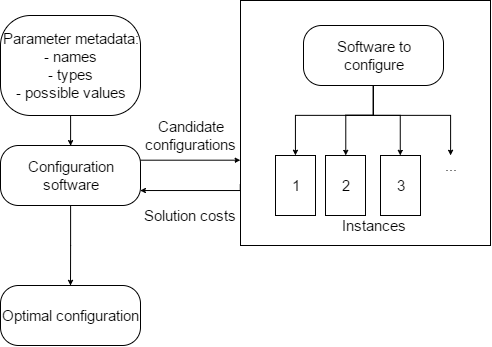
\includegraphics[scale=0.7]{configuration-top-level.png}
  \caption{Automatic configuration scheme}
  \label{fig:autoconf}
\end{figure}

Figure \ref{fig:autoconf} shows the configuration software and software to configure. Configuration script has parameter metadata at its disposal. Based on them, the configuration software runs the software to configure with candidate configurations according to some algorithm. After the configuration process finishes, the configuration software renders the best configurations obtained. In the most general software case there are two measures of the performance - solution quality (to maximize) and computation time (to minimize). This general approach is called an offline tuning. It introduces a learning stage on training instances before learning on the real-world instance set.


A widely used configuration algorithmic family is racing algorithms. The simplified algorithm is shown in \ref{lst:racing} and an illustration is in \ref{fig:irace}.


\begin{minipage}[c, breaklines=true]{0.95\textwidth}
\begin{lstlisting}[caption={General racing pseudo-code}, label={lst:racing}]
procedure racing
start with an initial candidate set Theta
repeat iterations I
	process an instance stream
	evaluate the candidates sequentially
	remove inferior candidates
until winner is selected or exit condition fulfilled
end
\end{lstlisting}
\end{minipage}


\begin{figure}
  \centering
    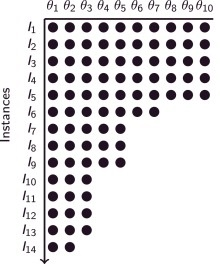
\includegraphics{irace.jpg}
  \caption{I-RACE execution illustration}
  \label{fig:irace}
\end{figure}


I-RACE (iterated race) configuration implementation was developed and described in \cite{iraceaac}. It was implemented in R with taking into account the parallel programming techniques and an initial candidate set-up. It is implemented as an offline tuning. That means, that the tuning is a separate preparatory process from the actual real-world problem application. The feature of the I-RACE is based on iterated generation of new configurations and removing of solutions with lower quality for further evaluating on the problem instances.

In order to tune the configurations that are sampled, I-RACE algorithms uses independent sampling distributions for each of the parameters. For numeric values those are normal distributions and discretely-defined distributions for the rest. The configuration biasing procedure is based on modifying the sampling distributions.

Iterated racing is an automatic configuration implementation that consists of three steps:

\begin{itemize}
\item Sampling new configurations according to a particular distribution.
\item Selecting the best configurations from the newly sampled ones by means of racing.
\item Updating the sampling distribution in order to bias the sampling towards the best configurations.
\end{itemize}

After new configurations are sampled comes the selection stage. At the configuration selection stage, I-RACE runs each of the configurations on a single problem instance from the predefined instance set. After each racing iteration the worst configurations are discarded. Then the rest of the configurations update parameter sampling distributions. The racing stops when the number of the survived configurations becomes small enough (defined by termination criteria).

Some I-RACE extensions can be applied. \textbf{Initial configurations} can be set before the run of the I-RACE. \textbf{Soft-restart} is used for preventing premature convergence. Such convergence may suppresses configuration diversity and, therefore some good configurations may be lost. This restart is triggered if the value of an ad hoc function of configuration distance is lower than a certain margin. Then reinitialization is applied to the elite configurations.


\chapter{Vehicle Routing Problem 5}


[correct formulas below under the VRP definition in the future] \newline

\section{Problem definition}

As a basis for VRP formulation variation we use the Classical Vehicle Routing Problem \cite{CORDEAU2007367}. However minor generalizations are actually implemented in the framework above the given formulation. \par

VRP is defined on a complete undirected graph $G=(V,E)$. A set of nodes $V=\{0,1,...,n\}$ is a union of all customer nodes $V\setminus\{0\}$ and a depot node $0$. Distance (a.k.a. travel cost or length or time) $c_e$ or $c_{ij}$ is assigned to each edge $e \in E = \{(i,j): i,j \in V, i<j\}$. Vehicle fleet is represented by $m$ identical vehicles, having a capacity $Q$ and total distance limit $L$.

Constraints are defined as follows:
\begin{enumerate}
\item Each customer is only visited by exactly one vehicle.
\item Each route starts and ends at the depot.
\item Total demand, that any vehicle provides does not exceed the capacity $Q$.
\item Total distance, that any vehicle passes on route does not exceed the limit L. 
\end{enumerate}

A proposed problem formulation is given below.

The decision variables $x_e$ are presented by an integer variable for each edge $e \in E$.

Let $r(S)$ be the minimum number of vehicles needed to serve the customers $S \subseteq V\setminus\{0\}, S \neq \emptyset$.

Let $\delta(S)=\{(i,j):i \in S, j \notin \textit{S or i} \notin S, j \in S\}$

Then we have a following integer linear programming problem:

\begin{equation}
\label{eq:cvrp_obj}
minimize {\sum\limits_{e \in E} c_ex_e} 
\end{equation}

\begin{equation}
\label{eq:cvrp_constr1}
{\sum\limits_{e \in \delta(i)} x_e = 2}, i \in V\setminus\{0\}
\end{equation}

\begin{equation}
\label{eq:cvrp_constr2}
{\sum\limits_{e \in \delta(0)} x_e = 2m},
\end{equation}

\begin{equation}
\label{eq:cvrp_constr3}
{\sum\limits_{e \in \delta(s)} x_e \geq 2r(S)},
\end{equation}

\begin{equation}
\label{eq:cvrp_constr4}
x_e \in \{0,1\}, e \notin \delta(0)
\end{equation}

\begin{equation}
\label{eq:cvrp_constr5}
x_e \in \{0,1,2\}, e \in \delta(0)
\end{equation}


However in addition to this definition one can apply several soothing generalizations:

\begin{enumerate}
\item \textbf{Non-symmetric matrix} can be considered, i.e. moving an edge one-way may have a different cost from moving backwards.
\item \textbf{Non-homogeneous vehicle fleet}. Every vehicle has its own maximum capacity and maximum distance.
\item A particular \textbf{vehicle may lack of maximum distance restriction}. In other words, maximum distance can be set to infinity.
\item \textbf{Open/closed problem variations can be also generalized}. Open VRP is a VRP variation, where a vehicle does not have to return to the depot. Closed is a variation, where it must return to the depot in any case. Generalization can be done at matrix definition step by setting all edges leaving from a customer to the depot to 0 in case of opened. On contrary, in closed VRP they are set to their actual travel cost.
\end{enumerate}


[tell about nearest neighbor heuristics, or not worthy?] \newline

\section{Candidate list}

Candidate list can severely boost performance. Similarly to TSP, \textbf{cl nearest neighbors} candidate lists can be used. For sake of optimization, these lists are computed once in the beginning of metaheuristcs execution and exploited during whole the run. Such a candidate list must be determined separately for every node.

During the preselection phase, the algorithm will examine the candidate list for the current node in the first place. In case if none of those will satisfy constraints (capacity, distance, already visited constraints), only then the nodes outside of the candidate list will be considered.

[basically explain all blue components from the UML]

\section{Heuristic values}

In VRP and TSP, one typically uses the inverted value of the distance between two nodes as the heuristics value, see \ref{eq:vrp_heuristic_value}. Thus, the selection phase will bias the tour edge towards shorter ones.

\begin{equation}
\label{eq:vrp_heuristic_value}
\eta_{edge} = 1 / c_{edge}
\end{equation}

\section{Local search}


[local search in VRP]

[perturbation double-bridge]





\chapter{Implementation 20-25}

[framework class-level description, no class diagram due to large size (however no descriptions for every class method. it's not a documentation)] \newline

[problem feasibility precheck]


\section{Preselection stage}

Generally in ACO optimization heuristics there are two ways of maintaining solution feasibility. First is two ensure solution \textbf{feasibility at every moment} of the run. Second is to \textbf{allow processing unfeasible solutions}, however trying to bias towards the components, that keep or likely to keep the solution feasible. Second is good for solving problems with complicated constraints that require a lot of computations in order to keep them feasible. In VRP however, we have decided to use the first approach. This will allow to avoid unnecessary construction of solutions, that are expected to be unfeasible beforehand. \par

Before applying selectors according to formulas \ref{eq:construction_classic}, \ref{eq:construction_maniezzo} or \ref{eq:construction_dorigo} one has to determine the possible solution components at the current construction step. Proposed preselection algorithm is shown in \ref{lst:preselection}. It selects all constraint non-violating edges. Among such constraints there are non-revisiting, not going to itself, not going to the depot edges. Out of those several are filtered out, such as the ones, who violate capacity constraint and distance constraint. In particular, we ensure condition $leftDistance >= dist(current;N) + dist(N;depot)$, since it does not make to go by a certain edge, if it will not be possible even to return to the depot from it. Neither it will be possible to return to the depot by going any farther from that node, which is ensured by triangle inequality property, that works in all VRP instances, that are based on Euclidean space. In case if none such node is found, then the vehicle returns directly to the depot from the current node.

In case if a candidate list is used, then the initial set is populated from this list, and the constraints are applied after.

\begin{minipage}[c, breaklines=true]{0.95\textwidth}
\begin{lstlisting}[caption={Solution component preselection pseudo-code}, label={lst:preselection}]
procedure preselection(currentNode)
	foreach non-visited non-loop non-depot-leading node N
		if leftCapacity >= demand(N)
			if leftDistance >= dist(current;N) + dist(N;depot)
				add component(current;N) to resultSet
			end
		end
	end
	
	if size(resultSet) == 0
		add component (current;depot) to result set
	end
		
	return resultSet
end
\end{lstlisting}
\end{minipage}


[mention the back-bone classes that provide generality and maintaining of VRP instance generality] \newline 

[framework parameters space] \newline

[mention unit testing???] \newline


\chapter{Experimental 20-25}

[public samples description, some publicly know plots] \newline

[configuration of i-race] \newline

[obtained result configuration for the framework] \newline

[description of the configuration]


\chapter{Conclusion 4-5}




\section{Literature}




\appendix

\backmatter

\printindex % use makeindex to generate the index



\bibliographystyle{plain}

\bibliography{biblio} %use bibtex to generate the bibliography

% BIBLIOGRAPHY DOES NOT WORK IN TEXMAKER, USE OVERLEAF FOR FINAL GENERATION

\end{document}
